	\subsubsection{Simulations for Fourier-Galerkin Method}
		
		Following the ideas in the previous section for the Fourier-Galerkin method, we will assume that the expansion of the solution of (\ref{IVP_Burgers}) is as follows
		\begin{align*}
			u(x, t) = \displaystyle \sum_{|n| \leq \infty} \hat{u}_n (t) \phi_n (x), \hspace{2mm} \hat{u}_n (t) = \frac{1}{2 \pi} \left\langle u (x, t), \phi_n (x) \right\rangle,  
		\end{align*}
		and as before $\phi_n (x) = e^{inx}$. \\
	
		Similarly, we consider the space $V_N = \hat{B}_N \cap H^2_p (\mathcal{D})$ where we will look for its truncated expansion given by
		\begin{align*}
			u_N (x, t) = \displaystyle \sum_{ |n| \leq N } \hat{u}_n (t) \phi_n (x), \hspace{2mm} \hat{u}_n (t) = \frac{1}{2 \pi} \left\langle u (x, t), \phi_n (x) \right\rangle, 
		\end{align*}  
		which we are going to force to satisfy the following
		\begin{align}
			\left\langle R_N, \phi_n \right\rangle = \left\langle \frac{\partial u_N}{\partial t} + \frac{1}{2} (u_N^2)_x - \alpha \frac{\partial^2 u_N}{\partial x^2}, \phi_n \right\rangle = 0, \hspace{2mm}  \hspace{2mm} \phi_n \in V_N, \hspace{2mm} \forall t > 0
		\end{align}
		or equivalently
		\begin{align*}
			\displaystyle \int_{I} \frac{\partial}{\partial t} u_N (x, t) \overline{\phi_n (x)} dx = \alpha \int_{I} \frac{\partial^2}{\partial x^2} u_N(x, t) \overline{\phi_n (x)} dx - \int_{I} \frac{1}{2} \frac{\partial}{\partial x} \left[ u_N(x, t) \right]^2 \overline{\phi_n (x)} dx   
		\end{align*}
		Since $u_N (x, t)$ and its derivatives are periodic in space, integrating by parts we obtain that
		\begin{align*}
			\displaystyle \int_{I} \frac{\partial}{\partial t} u_N (x, t) \overline{\phi_n (x)} dx = - \alpha \int_{I} \frac{\partial}{\partial x} u_N(x, t) \frac{\partial}{\partial x} \overline{\phi_n (x)} dx + \int_{I} \frac{1}{2} \left[ u_N(x, t) \right]^2 \frac{\partial}{\partial x} \overline{\phi_n (x)} dx   
		\end{align*} 
		
		Then writing again as an inner product
		\begin{align*}
			\left\langle \frac{\partial u_N}{\partial t}, \phi_n  \right\rangle = \left\langle - \alpha \frac{\partial u_N}{\partial x} + \frac{1}{2} [u_N]^2, \frac{\partial \phi_n}{\partial x}  \right\rangle
		\end{align*}
		and using the orthogonality $\langle \phi_l, \phi_n \rangle = 2 \pi \delta_{ln}$, for each $n$ fixed we have to
		\begin{align*}
			\left\langle \frac{\partial u_N}{\partial t}, \phi_n  \right\rangle = \left\langle \displaystyle \sum_{ |l| \leq N} \frac{d \hat{u}_l (t)}{dt} \phi_l, \phi_n  \right\rangle = 2 \pi \frac{d \hat{u}_n (t)}{dt}
		\end{align*}
		
		\noindent and for the other terms
		\begin{align*}
			\left\langle \frac{\partial u_N}{\partial x} - \frac{1}{2} [u_N]^2, \frac{\partial \phi_n}{\partial x}  \right\rangle = & \alpha \left\langle - i \displaystyle \sum_{ |l| \leq N} l \hat{u}_l (t) \phi_l, in \phi_n \right\rangle \\
			&+ \left\langle\frac{1}{2} \left( \sum_{ |p| \leq N} \hat{u}_p (t) \phi_p \right) \left( \sum_{ |q| \leq N} \hat{u}_q (t) \phi_q \right), in \phi_n \right\rangle \\
			=&  - \alpha n \left\langle  \displaystyle \sum_{ |l| \leq N} l \hat{u}_l (t) \phi_l, \phi_n \right\rangle - \frac{in}{2} \left\langle \sum_{ |p| \leq N} \sum_{ |q| \leq N} \hat{u}_p (t) \hat{u}_q (t) \phi_{p + q}, \phi_n \right \rangle \\
			=& -2 \pi \alpha n^2 \hat{u}_n (t) - in \pi \sum_{ p + q = n} \hat{u}_p (t) \hat{u}_q (t), \hspace{2mm} |q|, |p| \leq N.
		\end{align*}
		
		\noindent Therefore, using the linear transformation from $\mathcal{D}_p = [0, 2 \pi]$ to $\mathcal{D} = [x_L, x_R]$ given by $x = P z + x_L$ to escalate the problem, where $P = \frac{x_R - x_L}{2 \pi}$ and $z \in \mathcal{D}_p$, we have the following system of nonlinear ordinary differential equations
		\begin{align}
		\label{Galerkin_Nonlinear}	
			\frac{d \hat{u}_n (t)}{dt} = - \alpha P^2 n^2 \hat{u}_n (t) - \frac{in}{2} P \sum_{ p + q = n} \hat{u}_p (t) \hat{u}_q (t), \hspace{2mm} |q|, |p| \leq N, 
		\end{align}
		or equivalently
		\begin{align*}
			\frac{d \hat{u}_n (t)}{dt} = - \alpha P^2 n^2 \hat{u}_n (t) - \frac{in}{2} P \sum_{|q| \leq N} \hat{u}_{n - q} (t) \hat{u}_q (t), \hspace{2mm} |n| \leq N, 
		\end{align*}
		which is solved using the initial condition of the original projected problem on the space $V_N$, that is,
		\begin{align*}
			\mathcal{P}_N u_0 = \displaystyle \sum_{|n| \leq N} a_n \phi_n (x), \hspace{2mm} a_n = \frac{1}{2 \pi} \langle u_0 (x), \phi_n (x) \rangle.   
		\end{align*}
		
		This problem can be treated in different ways and, in this work, we will develop it with the following approach. First, let's discard the terms $\hat{u}_q$ such that $|q| > N$ on the right side of the equation above, to get the following
		\begin{align*}
			\frac{d \hat{u}_n (t)}{dt} =  -\alpha P^2 n^2 \hat{u}_n (t) - \frac{in}{2} P \sum_{|q| \leq N} \hat{u}_{n - q} (t) \hat{u}_q (t), \hspace{2mm} |n - q| \leq N , 
		\end{align*}
		which is a system of $2N + 1$ equations. \\
		
		There is a wide variety of numerical methods to solve the above problem, and since this is not linear, it is not easy to justify choosing an appropriate method, since advanced knowledge of numerical analysis is required to investigate its characteristics. The way to choose a candidate method is by investigating its numerical stability, which guarantees that the numerical solution does not explode towards infinity and that it is at least bounded. \\
		
		In general, explicit methods are not suitable for nonlinear problems and are commonly handled by implicit methods. To show the implementation, and in addition to looking at its most relevant characteristics, we will solve the problem using Euler's implicit method. First, note that when $n = 0$ we have $\hat{u}_0 (t) = \hat{u}_0 (0)$, and that the nonlinear term involves the term $\hat{u}_n$ only when $q = 0$. So, using the integrating factor $e^{\lambda_n t}$ with $\lambda_n = \alpha P^2 n^2 + \frac{in}{2} P \hat{u}_0 (0) $ we can obtain the following formulation
		\begin{align*}
			\frac{d \left[ e^{\lambda_n t} \right]  \hat{u}_n (t)}{dt} = - \frac{in}{2} P e^{ \lambda_n t} \left[ \hat{u}_0 (0) \hat{u}_n (t) + \sum_{\substack{|q|\leq N \\ q \neq 0, n}} \hat{u}_{n - q} (t) \hat{u}_q (t) \right],
		\end{align*}	
		and its solution using implicit Euler
		\begin{align*}
			\hat{u}^{j+1}_n = e^{- \lambda_n \Delta t} \left[ \hat{u}^j_n - \Delta t \frac{in}{2} P \sum_{\substack{|q|\leq N \\ q \neq 0, n}} \hat{u}^{j}_{n - q} \hat{u}^{j}_q \right] - \Delta t \frac{in}{2} P \hat{u}_0 (0) \hat{u}^{j+1}_n, 
		\end{align*}
		and then solving for the term $\hat{u}^{j + 1}_n$ to obtain
		\begin{align*}
			\hat{u}^{j+1}_n &= \frac{ e^{- \lambda_n \Delta t}}{ 1 + \Delta t \frac{in}{2} P \hat{u}_0 (0) } \left[ \hat{u}^j_n - \Delta t \frac{in}{2} P \sum_{\substack{|q|\leq N \\ q \neq 0, n}} \hat{u}^{j}_{n - q} \hat{u}^{j}_q \right].   
		\end{align*}	
		
		Furthermore, using this formulation repeatedly for each $j$ gives us
		\begin{align}
		\label{Galerkin_Euler}
			\hat{u}^{j+1}_n &= \left[ \frac{ e^{- \lambda_n \Delta t}}{ 1 + \Delta t \frac{in}{2} P \hat{u}_0 (0) } \right]^{j+1} \hat{u}^0_n - \Delta t \frac{in}{2} P \sum_{k=1}^{j+1} \left[ \frac{ e^{- \lambda_n \Delta t}}{ 1 + \Delta t \frac{in}{2} P \hat{u}_0 (0) } \right]^{k}  \sum_{\substack{|q|\leq N \\ q \neq 0, n}} \hat{u}^{j+1-k}_{n - q} \hat{u}^{j+1-k}_q
		\end{align}
		Now, we will proceed to describe the steps necessary to implement the method based on the above. The simulations we are going to show were based on the formulation (\ref{Galerkin_Euler}), taking advantage of the fast Fourier transformation to calculate the coefficients $\hat{u}_n$, since it allows us to go from physical space to the space of Fourier and conversely. Also, it is worth mentioning that the codes used in this work can be found at \url{https://github.com/alanmatzumiya/pySpectralPDE.git}. \\ 
		
		To carry out these numerical experiments it was necessary to follow the following steps:
		\begin{enumerate}
			\item Set the intervals to consider, $[x_L, x_R]$ for physical space and $[t_0, t_f]$ for time, and give an initial condition function $u_0$. It is also necessary to choose the value of $N$, and another for the parameter $\alpha$. 
			
			\item We proceed to calculate the points in the spatial grid where we want to obtain the solution, and for this, we define the points $z_i \in [0, 2 \pi]$ as
			\begin{align*}
				z_i = \frac{2 \pi i}{N}, \hspace{2mm} i = 0, 1, \dots, N
			\end{align*}
			which are used to obtain the points $x_i \in [x_L, x_R]$
			\begin{align*}
				x_i = P z_i + x_L, \hspace{2mm} P = \frac{x_R - x_L}{2 \pi}
			\end{align*}
			
			To obtain the points $t_j \in [t_0, t_f]$, we define the sequence $j = 0, 1, \dots, M$, for some positive $M$, and calculate the following
			\begin{align*}
				t_j = t_0 + j \Delta t, \hspace{2mm} \Delta t = \frac{t_f - t_0}{M} 
			\end{align*}
			
			The values $| n | = 0, 1, \dots, N $ must be established to calculate $in, n^2$, which are required to approximate the derivatives.
			 
			\item Calculate the coefficients $\hat{u}_0$ of the initial condition function $u_0$, using the fast Fourier transformation based on the already fixed spatial grid. So, it is possible to start the recursive rule given by (\ref{Galerkin_Euler}) for every $t_j$.
			
			\item Finally, the approximation obtained is evaluated using the equation given by
			\begin{align*}
				u_N(x, t_j) = \displaystyle \sum_{|n| \leq N} \hat{u}_n (t_j) e^{inx}.
			\end{align*}
		\end{enumerate}
		
		For the numerical study, we will establish the following initial condition
		\begin{align}
			\label{IC}
			u_0 (x) = e^{0.05 x^2}, \hspace{3mm} x \in [x_L, x_R] 
		\end{align}	
		
		To compare results, we will use the approximation given by (\ref{Exact_Solution_Approximation}) as the exact solution. In the figure \ref{Galerkin_alphas} shows the maximum distance over every $t \in [0, 100]$ between the exact solution and its approximations given by (\ref{Galerkin_Euler}) for $N = 2^m$, $m = 4, \dots, 12$, $\Delta t = 1.0 \times 10^{-5}$, and different values of $\alpha$. Furthermore, in Tables \ref{Galerkin_tabla_L2_alpha=1} and \ref{Galerkin_tabla_max_alpha=1}, we can see the numerical values ​​of these distances for different configurations of $N$ and $\Delta t$. Similarly, in Tables \ref{Galerkin_tabla_L2_alpha=005} and \ref{Galerkin_tabla_max_alpha=005} but for $\alpha = 0.005$.
	
	\begin{figure}[H]
		\centering
		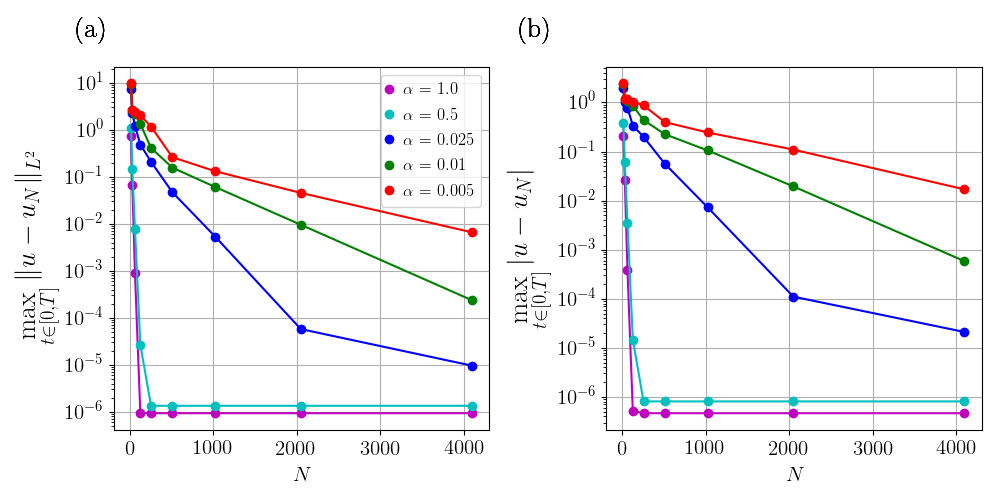
\includegraphics[width=15cm]{burgers_equation/deterministic/numerical_experiments/viscid/figures/galerkin/alphas_Error_N.png}
		\caption{(a) $L^2$-norm between the exact solution and its approximations using Galerkin method. (b) Max norm between the exact solution and its approximations.}
		\label{Galerkin_alphas}
	\end{figure}
	\newpage
	\begin{figure}[H]
		\centering
		\caption{Numerical solution for (\ref{IVP_Burgers}) using (\ref{Galerkin_Euler}) with $\alpha = 1.0$, $N=2048$, and $\Delta t = 1.0 \times 10^{-5}$.}
		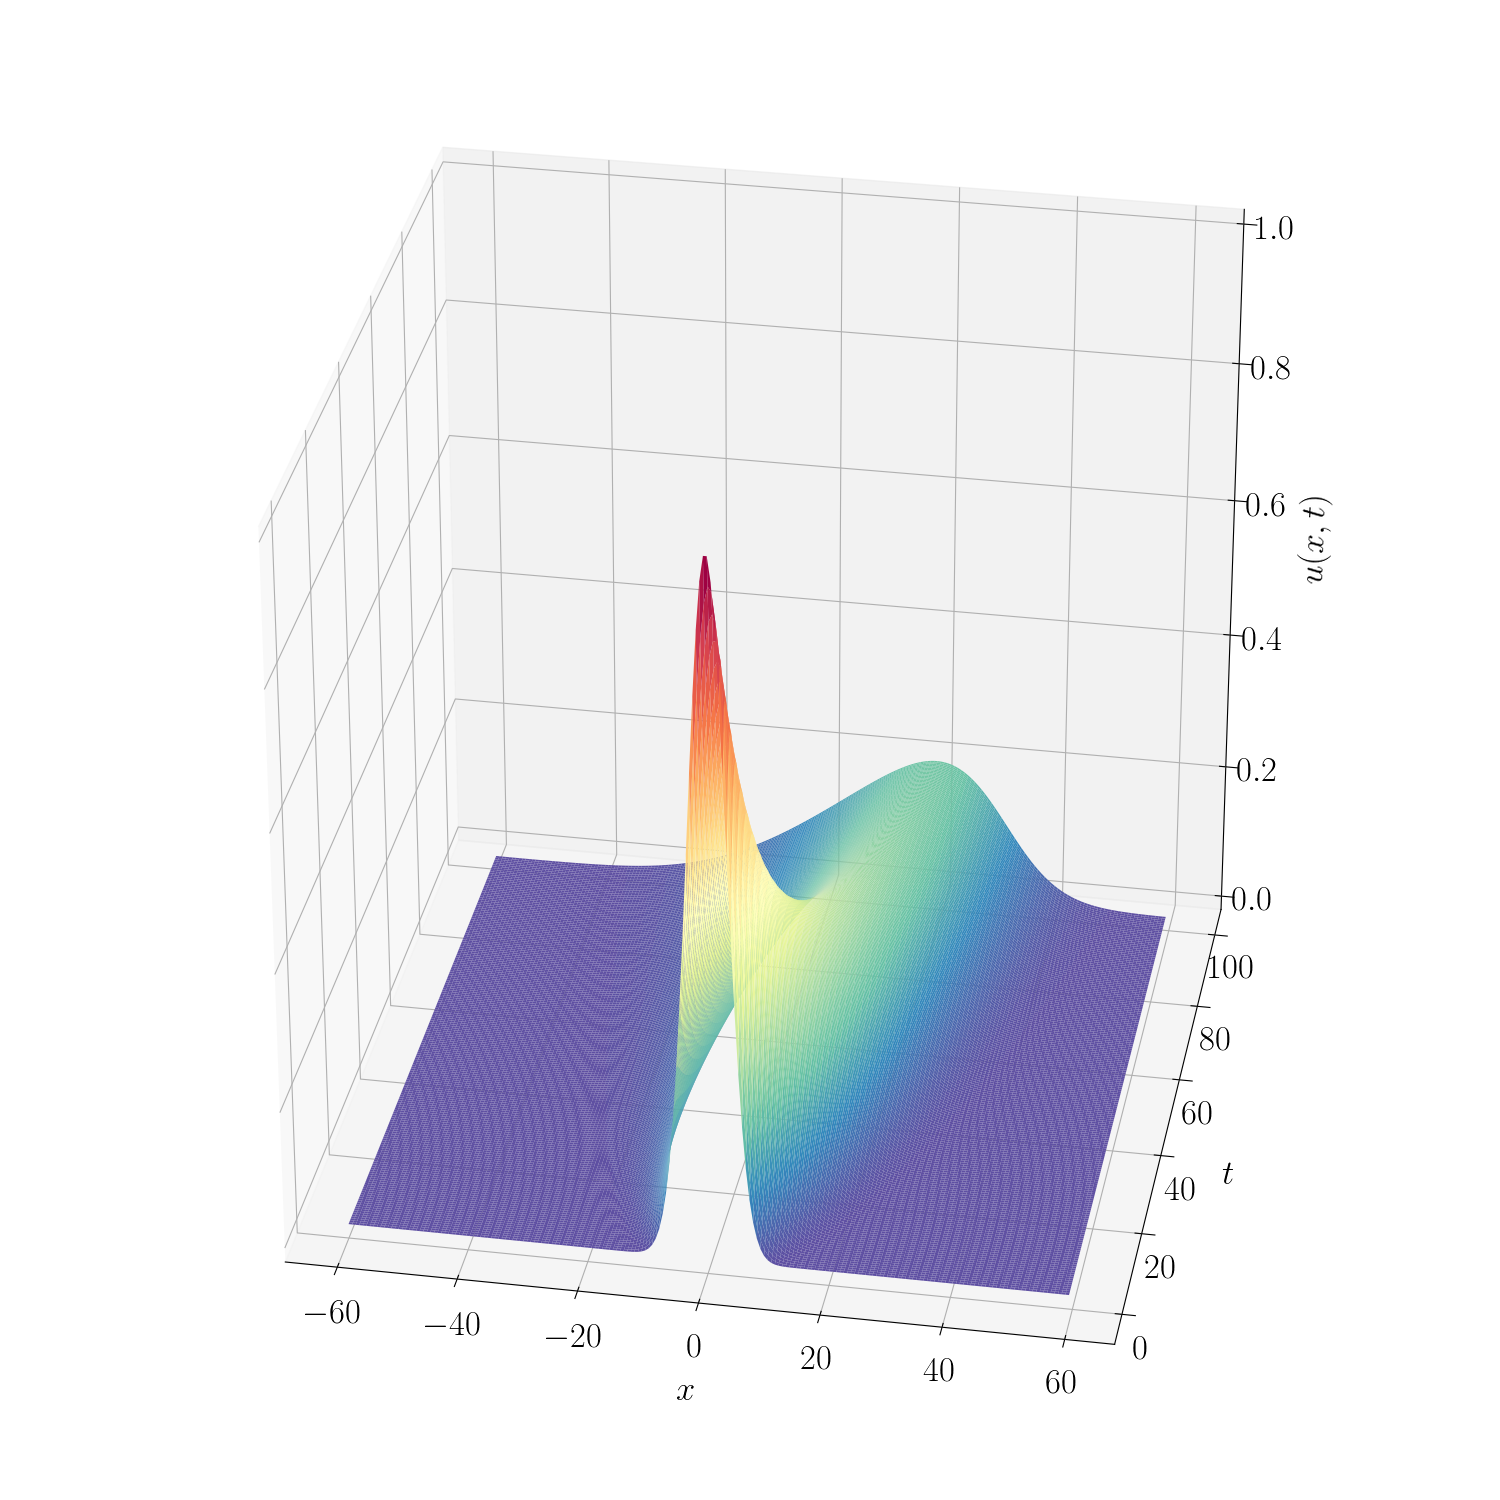
\includegraphics[width=12cm]{burgers_equation/deterministic/numerical_experiments/viscid/figures/galerkin/Numerical_Solution_alpha=1.png}
		\label{Galerkin_alpha=1}
		\caption{Numerical solution for (\ref{IVP_Burgers}) using (\ref{Galerkin_Euler}) at the time $T = 100$ with $\alpha = 1.0$, and $\Delta t = 1.0 \times 10^{-5}$. (b) Point-wise error of approximation}
		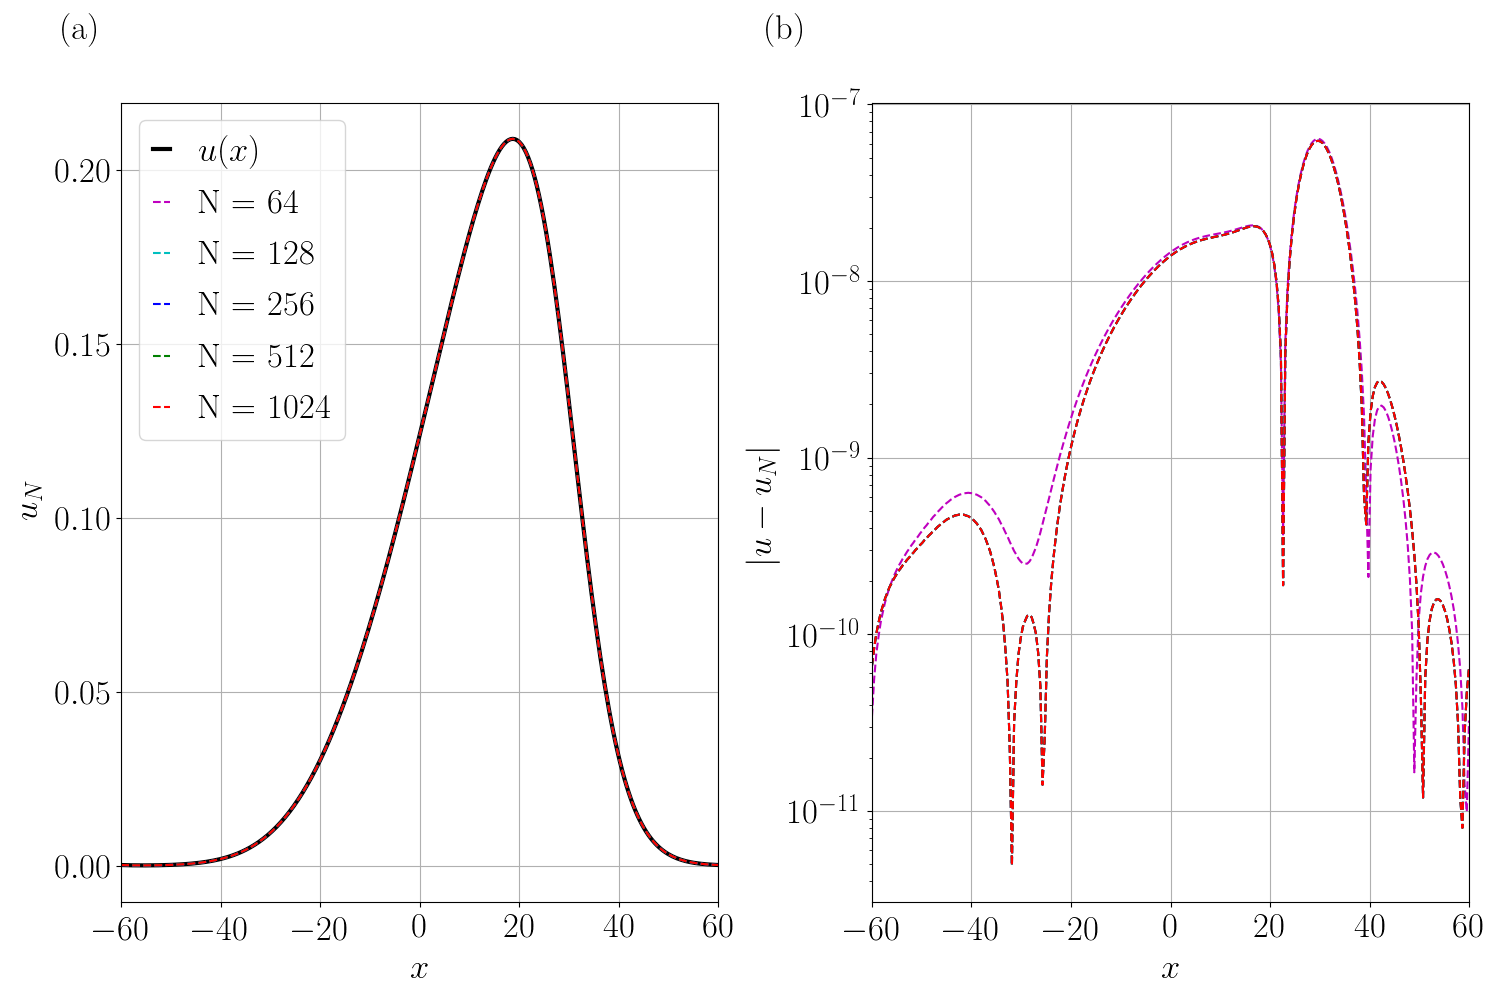
\includegraphics[width=12.5cm]{burgers_equation/deterministic/numerical_experiments/viscid/figures/galerkin/Numerical_Solution_alpha=1_T=100.png}
		\label{Galerkin_alpha=1_T}
	\end{figure}
	\begin{table}[H]
		\begin{tabular}{lcccc}
			\toprule
			\multicolumn{1}{c}{\textbf{Expansion}} & \multicolumn{4}{c}{\textbf{Error}} \\
			$\hspace{9mm}N$ & $\Delta t=1\times 10^{-2}$ & $\Delta t=1\times 10^{-3}$ & $\Delta t=1\times 10^{-4}$ & $\Delta t=1\times 10^{-5}$ \\
			\midrule
			\hspace{7mm} 16 & 0.72504    & 0.72504    & 0.72504    & 0.72504    \\
			\midrule
			\hspace{7mm} 32 & 6.90249 $\times 10 ^{-2}$   & 6.88052 $\times 10 ^{-2}$   & 6.87838 $\times 10 ^{-2}$   & 6.87816 $\times 10 ^{-2}$   \\
			\midrule
			\hspace{7mm} 64 & 1.23827 $\times 10 ^{-3}$  & 8.85367 $\times 10 ^{-4}$ & 8.80521 $\times 10 ^{-4}$ & 8.80410 $\times 10 ^{-4}$  \\
			\midrule
			\hspace{7mm} 128 & 9.43454 $\times 10 ^{-4}$ & 9.41793 $\times 10 ^{-5}$ & 9.41148 $\times 10 ^{-6}$ & 9.41827 $\times 10 ^{-7}$  \\
			\midrule
			\hspace{7mm} 256 & 9.43454 $\times 10 ^{-4}$ & 9.41793 $\times 10 ^{-5}$ & 9.41109 $\times 10 ^{-6}$ & 9.36411 $\times 10 ^{-7}$ \\
			\midrule
			\hspace{7mm} 512 & 9.43454 $\times 10 ^{-4}$ & 9.41793 $\times 10 ^{-5}$ & 9.41109 $\times 10 ^{-6}$ & 9.36411 $\times 10 ^{-7}$ \\
			\midrule
			\hspace{7mm} 1024 & $\ast$ & 9.41793 $\times 10^{-5}$ & 9.41109 $\times 10^{-6}$ & 9.36411 $\times 10^{-7}$              \\
			\midrule
			\hspace{7mm} 2048 & $\ast$ & $\ast$ & 9.41109 $\times 10^{-6}$ & 9.36411 $\times 10^{-7}$   \\
			\bottomrule
		\end{tabular}
		\caption{Error using $L^2$-norm with $\alpha = 1.0$}
		\label{Galerkin_tabla_L2_alpha=1}
		\vspace{1cm}
		\begin{tabular}{lcccc}
			\toprule
			\multicolumn{1}{c}{\textbf{Expansion}} & \multicolumn{4}{c}{\textbf{Error}} \\
			$\hspace{9mm}N$ & $\Delta t=1\times 10^{-2}$ & $\Delta t=1\times 10^{-3}$ & $\Delta t=1\times 10^{-4}$ & $\Delta t=1\times 10^{-5}$ \\
			\midrule
			\hspace{7mm} 16 & 0.203363    & 0.203333    & 0.203331    & 0.20333     \\
			\midrule
			\hspace{7mm} 32 & 2.64192 $\times 10 ^{-2}$   & 2.6248 $\times 10 ^{-2}$    & 2.62491 $\times 10 ^{-2}$  & 2.62492 $\times 10 ^{-2}$   \\
			\midrule
			\hspace{7mm} 64 & 6.93001 $\times 10 ^{-4}$ & 4.11641 $\times 10 ^{-4}$ & 3.85563 $\times 10 ^{-4}$ & 3.82972 $\times 10 ^{-4}$ \\
			\midrule
			\hspace{7mm} 128 & 4.74934 $\times 10 ^{-4}$ & 4.73649 $\times 10 ^{-5}$ & 4.74295 $\times 10 ^{-6}$ & 5.16105 $\times 10 ^{-7}$ \\
			\midrule
			\hspace{7mm} 256 & 4.74936 $\times 10 ^{-4}$ & 4.7368 $\times 10 ^{-5}$  & 4.72569 $\times 10 ^{-6}$ & 4.64922 $\times 10 ^{-7}$ \\
			\midrule
			\hspace{7mm} 512 & 4.74936 $\times 10 ^{-4}$ & 4.7368 $\times 10 ^{-5}$  & 4.72569 $\times 10 ^{-6}$ & 4.64922 $\times 10 ^{-4}$ \\
			\midrule
			\hspace{7mm} 1024 & * & 4.7368 $\times 10 ^{-5}$  & 4.72569 $\times 10 ^{-6}$ & 4.64922 $\times 10 ^{-7}$ \\
			\midrule
			\hspace{7mm} 2048 & * & * & 4.72569 $\times 10 ^{-6}$ & 4.64922 $\times 10 ^{-7}$ \\
			\bottomrule
		\end{tabular}
		\caption{Error using Max norm with $\alpha = 1.0$}
		\label{Galerkin_tabla_max_alpha=1}
	\end{table}

	\begin{figure}[H]
		\centering
		\caption{Numerical solution for (\ref{IVP_Burgers}) using (\ref{Galerkin_Euler}) with $\alpha = 0.005$, $N=2048$, and $\Delta t = 1.0 \times 10^{-5}$.}
		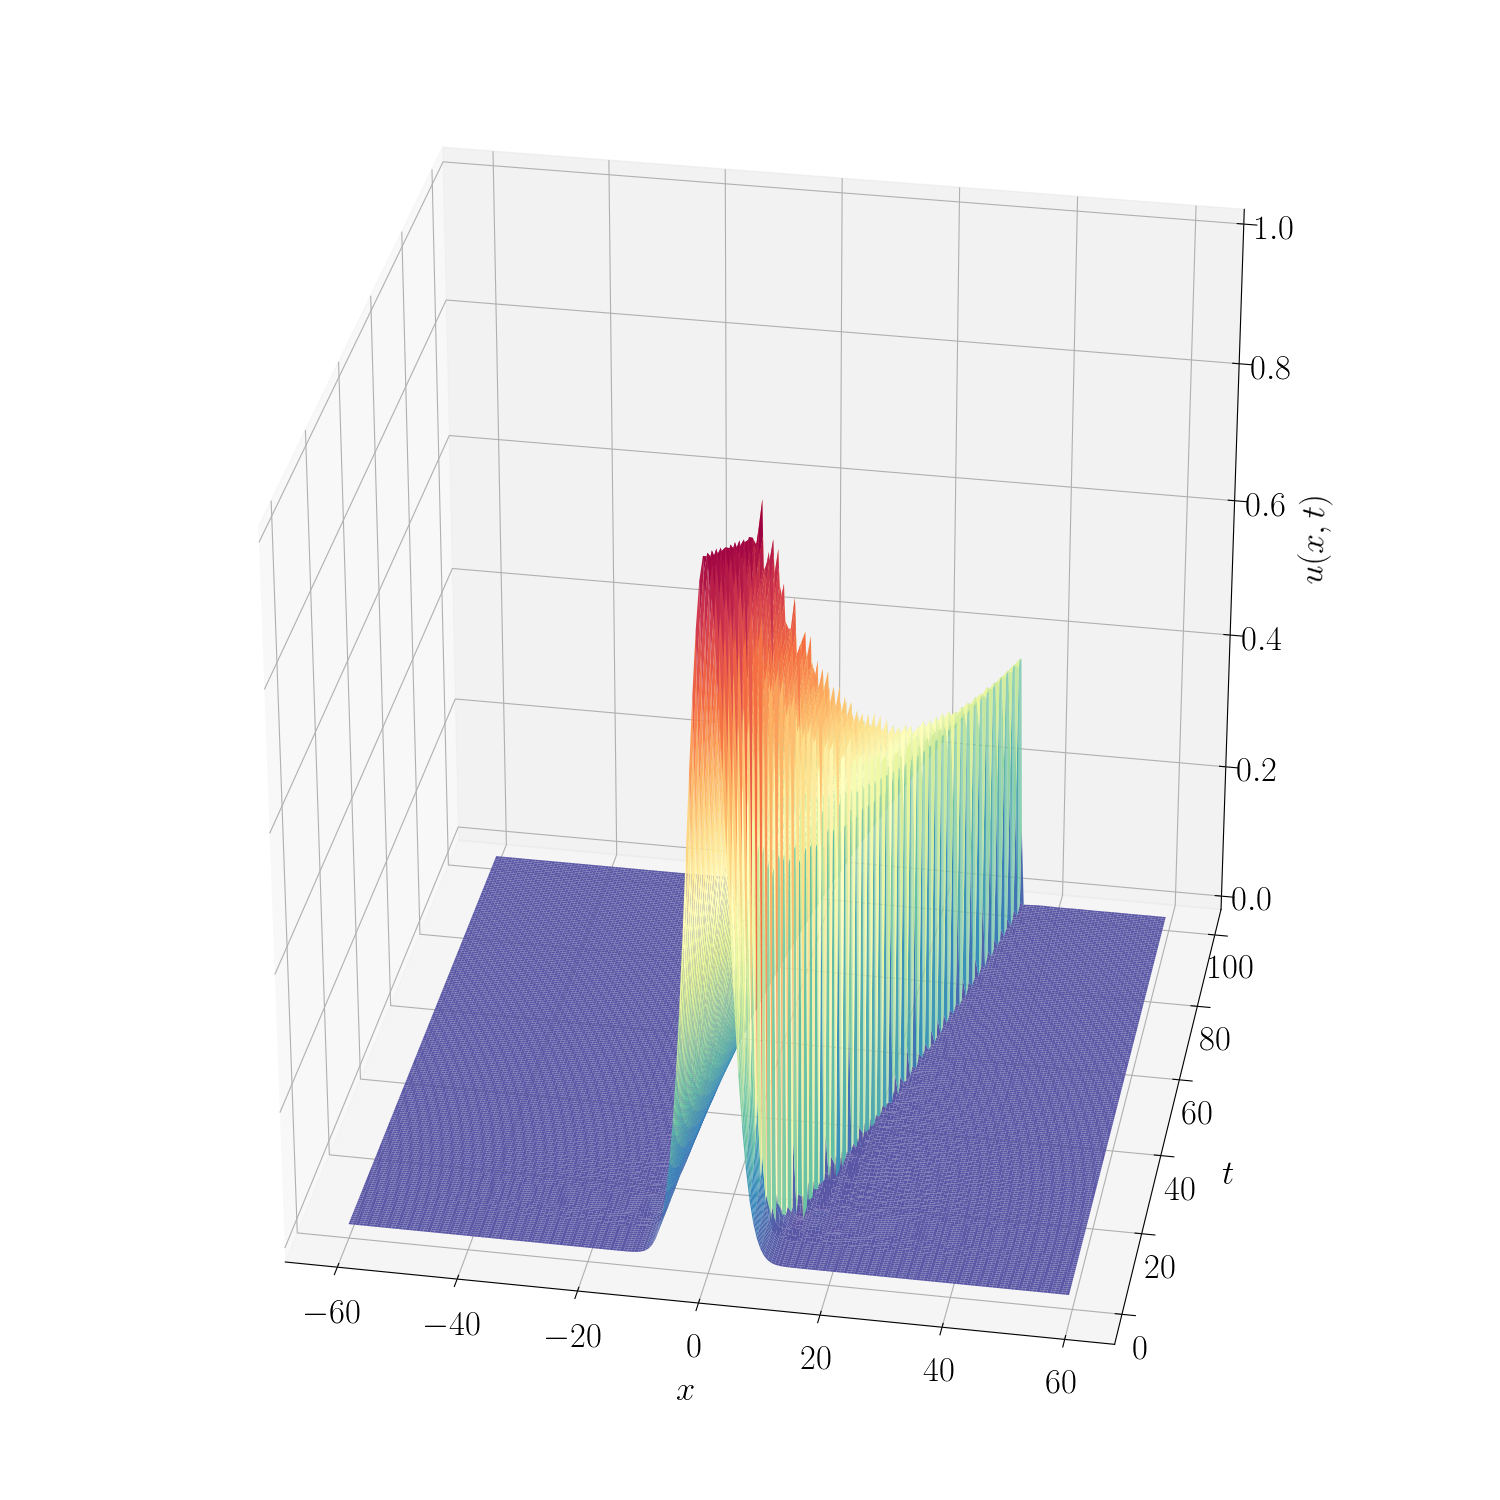
\includegraphics[width=12cm]{burgers_equation/deterministic/numerical_experiments/viscid/figures/galerkin/Numerical_Solution_alpha=0005.png}
		\caption{Numerical solution for (\ref{IVP_Burgers}) using (\ref{Galerkin_Euler}) at the time $T = 100$ with $\alpha = 1.0$, and $\Delta t = 1.0 \times 10^{-5}$. (b) Point-wise error of approximation}
		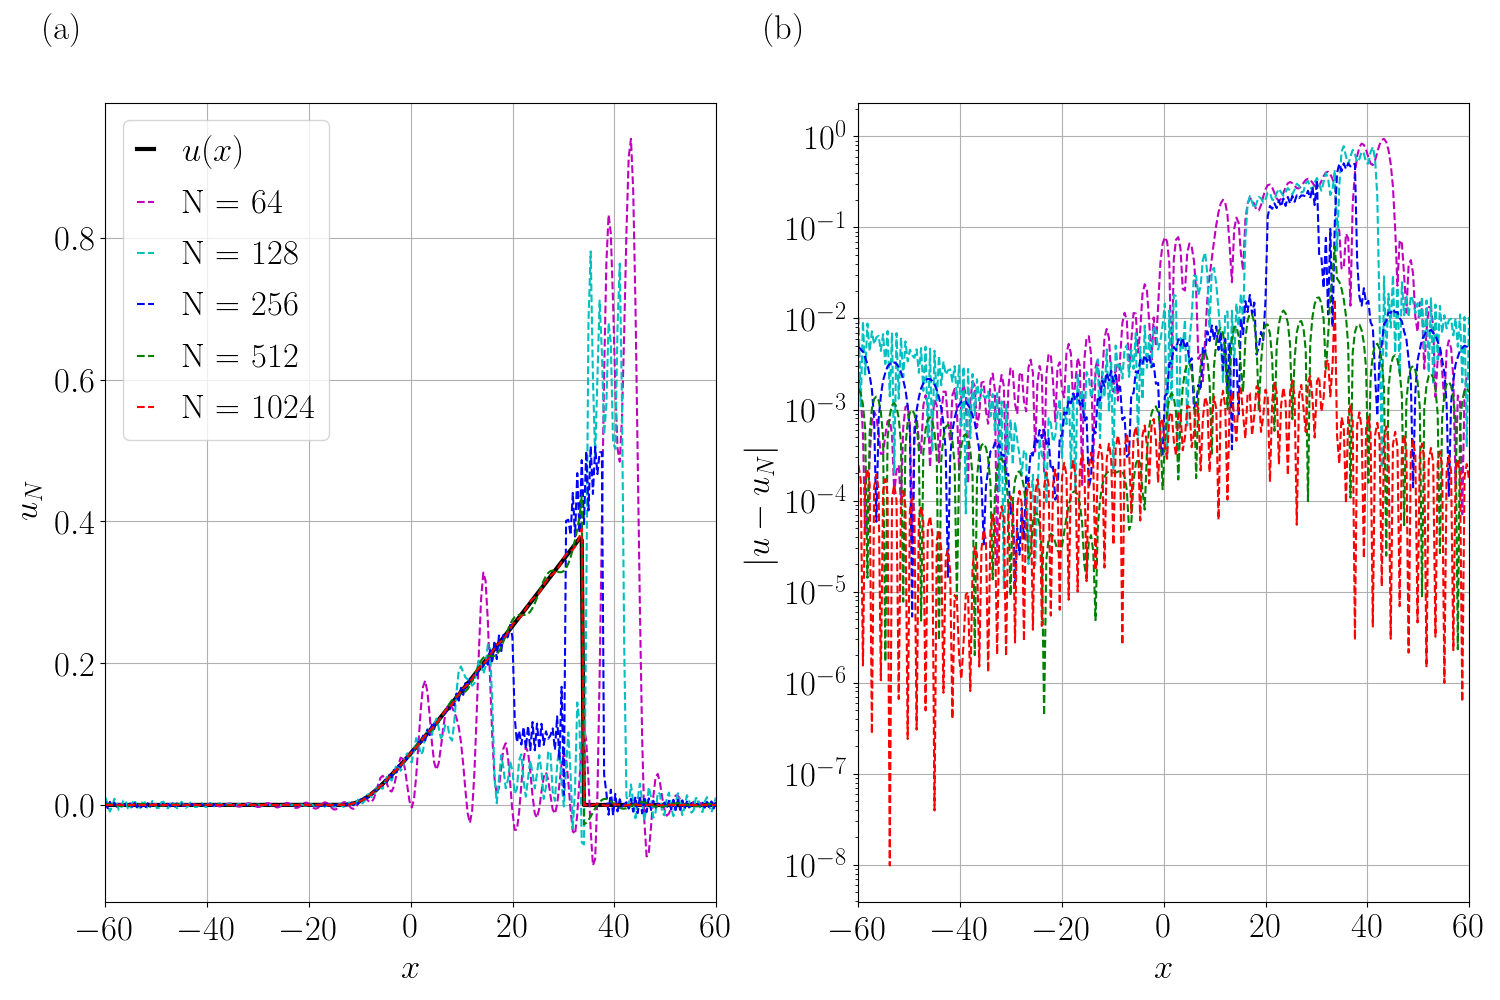
\includegraphics[width=12.5cm]{burgers_equation/deterministic/numerical_experiments/viscid/figures/galerkin/Numerical_Solution_alpha=0005_T=100.png}
		\label{Galerkin_alpha=005_T}
	\end{figure}
	
	\begin{table}[H]
	\begin{tabular}{lcccc}
		\toprule
		\multicolumn{1}{c}{\textbf{Expansion}} & \multicolumn{4}{c}{\textbf{Error}} \\
		$\hspace{9mm}N$ & $\Delta t=1\times 10^{-2}$ & $\Delta t=1\times 10^{-3}$ & $\Delta t=1\times 10^{-4}$ & $\Delta t=1\times 10^{-5}$ \\
		\midrule
		\hspace{7mm} 16 & 9.95328   & 9.91901    & 9.91597    & 9.91567    \\
		\midrule
		\hspace{7mm} 32 & 2.72607   & 2.70558    & 2.70347    & 2.70326    \\
		\midrule
		\hspace{7mm} 64 & 2.50343   & 2.45988    & 2.45543    & 2.45497    \\
		\midrule
		\hspace{7mm} 128 & 2.16142   & 2.06992    & 2.05918    & 2.05795    \\
		\midrule
		\hspace{7mm} 256 & 1.3658    & 1.19385    & 1.17602    & 1.17412    \\
		\midrule
		\hspace{7mm} 512 & 0.339826  & 0.265843   & 0.262164   & 0.261805   \\
		\midrule
		\hspace{7mm} 1024 & 0.161405  & 0.133743   & 0.131882   & 0.131699   \\
		\midrule
		\hspace{7mm} 2048 & 6.50292 $\times 10^{-2}$ & 4.70602 $\times 10^{-2}$ & 4.57371 $\times 10^{-2}$  & 4.56090 $\times 10^{-2}$  \\
		\bottomrule
	\end{tabular}
	\caption{Error using $L^2$-norm with $\alpha = 0.005$}
	\label{Galerkin_tabla_L2_alpha=005}
	\vspace{1cm}
	\begin{tabular}{lcccc}
		\toprule
		\multicolumn{1}{c}{\textbf{Expansion}} & \multicolumn{4}{c}{\textbf{Error}} \\
		$\hspace{9mm}N$ & $\Delta t=1\times 10^{-2}$ & $\Delta t=1\times 10^{-3}$ & $\Delta t=1\times 10^{-4}$ & $\Delta t=1\times 10^{-5}$ \\
		\midrule
		\hspace{7mm} 16 & 2.50002  & 2.48992   & 2.48891   & 2.48881   \\
		\midrule
		\hspace{7mm} 32 & 1.21263  & 1.20544   & 1.2047    & 1.20463   \\
		\midrule
		\hspace{7mm} 64 & 1.21269  & 1.17736   & 1.17517   & 1.17495   \\
		\midrule
		\hspace{7mm} 128 & 1.10164  & 1.03493   & 1.03093   & 1.03048   \\
		\midrule
		\hspace{7mm} 256 & 0.954369 & 0.881472  & 0.873392  & 0.87259   \\
		\midrule
		\hspace{7mm} 512 & 0.665071 & 0.418735  & 0.398664  & 0.396931  \\
		\midrule
		\hspace{7mm} 1024 & 0.241841 & 0.244188  & 0.244437  & 0.244461  \\
		\midrule
		\hspace{7mm} 2048 & 0.133067 & 0.104675  & 0.109151  & 0.109596  \\
		\bottomrule
	\end{tabular}
	\caption{Error using Max norm with $\alpha =0.005$}
	\label{Galerkin_tabla_max_alpha=005}
	\end{table}
	
	\newpage
